% Options for packages loaded elsewhere
\PassOptionsToPackage{unicode}{hyperref}
\PassOptionsToPackage{hyphens}{url}
%
\documentclass[
]{book}
\title{环境数据分析与可视化}
\author{谭巧国}
\date{2022-06-05}

\usepackage{amsmath,amssymb}
\usepackage{lmodern}
\usepackage{iftex}
\ifPDFTeX
  \usepackage[T1]{fontenc}
  \usepackage[utf8]{inputenc}
  \usepackage{textcomp} % provide euro and other symbols
\else % if luatex or xetex
  \usepackage{unicode-math}
  \defaultfontfeatures{Scale=MatchLowercase}
  \defaultfontfeatures[\rmfamily]{Ligatures=TeX,Scale=1}
\fi
% Use upquote if available, for straight quotes in verbatim environments
\IfFileExists{upquote.sty}{\usepackage{upquote}}{}
\IfFileExists{microtype.sty}{% use microtype if available
  \usepackage[]{microtype}
  \UseMicrotypeSet[protrusion]{basicmath} % disable protrusion for tt fonts
}{}
\makeatletter
\@ifundefined{KOMAClassName}{% if non-KOMA class
  \IfFileExists{parskip.sty}{%
    \usepackage{parskip}
  }{% else
    \setlength{\parindent}{0pt}
    \setlength{\parskip}{6pt plus 2pt minus 1pt}}
}{% if KOMA class
  \KOMAoptions{parskip=half}}
\makeatother
\usepackage{xcolor}
\IfFileExists{xurl.sty}{\usepackage{xurl}}{} % add URL line breaks if available
\IfFileExists{bookmark.sty}{\usepackage{bookmark}}{\usepackage{hyperref}}
\hypersetup{
  pdftitle={环境数据分析与可视化},
  pdfauthor={谭巧国},
  hidelinks,
  pdfcreator={LaTeX via pandoc}}
\urlstyle{same} % disable monospaced font for URLs
\usepackage{color}
\usepackage{fancyvrb}
\newcommand{\VerbBar}{|}
\newcommand{\VERB}{\Verb[commandchars=\\\{\}]}
\DefineVerbatimEnvironment{Highlighting}{Verbatim}{commandchars=\\\{\}}
% Add ',fontsize=\small' for more characters per line
\usepackage{framed}
\definecolor{shadecolor}{RGB}{248,248,248}
\newenvironment{Shaded}{\begin{snugshade}}{\end{snugshade}}
\newcommand{\AlertTok}[1]{\textcolor[rgb]{0.94,0.16,0.16}{#1}}
\newcommand{\AnnotationTok}[1]{\textcolor[rgb]{0.56,0.35,0.01}{\textbf{\textit{#1}}}}
\newcommand{\AttributeTok}[1]{\textcolor[rgb]{0.77,0.63,0.00}{#1}}
\newcommand{\BaseNTok}[1]{\textcolor[rgb]{0.00,0.00,0.81}{#1}}
\newcommand{\BuiltInTok}[1]{#1}
\newcommand{\CharTok}[1]{\textcolor[rgb]{0.31,0.60,0.02}{#1}}
\newcommand{\CommentTok}[1]{\textcolor[rgb]{0.56,0.35,0.01}{\textit{#1}}}
\newcommand{\CommentVarTok}[1]{\textcolor[rgb]{0.56,0.35,0.01}{\textbf{\textit{#1}}}}
\newcommand{\ConstantTok}[1]{\textcolor[rgb]{0.00,0.00,0.00}{#1}}
\newcommand{\ControlFlowTok}[1]{\textcolor[rgb]{0.13,0.29,0.53}{\textbf{#1}}}
\newcommand{\DataTypeTok}[1]{\textcolor[rgb]{0.13,0.29,0.53}{#1}}
\newcommand{\DecValTok}[1]{\textcolor[rgb]{0.00,0.00,0.81}{#1}}
\newcommand{\DocumentationTok}[1]{\textcolor[rgb]{0.56,0.35,0.01}{\textbf{\textit{#1}}}}
\newcommand{\ErrorTok}[1]{\textcolor[rgb]{0.64,0.00,0.00}{\textbf{#1}}}
\newcommand{\ExtensionTok}[1]{#1}
\newcommand{\FloatTok}[1]{\textcolor[rgb]{0.00,0.00,0.81}{#1}}
\newcommand{\FunctionTok}[1]{\textcolor[rgb]{0.00,0.00,0.00}{#1}}
\newcommand{\ImportTok}[1]{#1}
\newcommand{\InformationTok}[1]{\textcolor[rgb]{0.56,0.35,0.01}{\textbf{\textit{#1}}}}
\newcommand{\KeywordTok}[1]{\textcolor[rgb]{0.13,0.29,0.53}{\textbf{#1}}}
\newcommand{\NormalTok}[1]{#1}
\newcommand{\OperatorTok}[1]{\textcolor[rgb]{0.81,0.36,0.00}{\textbf{#1}}}
\newcommand{\OtherTok}[1]{\textcolor[rgb]{0.56,0.35,0.01}{#1}}
\newcommand{\PreprocessorTok}[1]{\textcolor[rgb]{0.56,0.35,0.01}{\textit{#1}}}
\newcommand{\RegionMarkerTok}[1]{#1}
\newcommand{\SpecialCharTok}[1]{\textcolor[rgb]{0.00,0.00,0.00}{#1}}
\newcommand{\SpecialStringTok}[1]{\textcolor[rgb]{0.31,0.60,0.02}{#1}}
\newcommand{\StringTok}[1]{\textcolor[rgb]{0.31,0.60,0.02}{#1}}
\newcommand{\VariableTok}[1]{\textcolor[rgb]{0.00,0.00,0.00}{#1}}
\newcommand{\VerbatimStringTok}[1]{\textcolor[rgb]{0.31,0.60,0.02}{#1}}
\newcommand{\WarningTok}[1]{\textcolor[rgb]{0.56,0.35,0.01}{\textbf{\textit{#1}}}}
\usepackage{longtable,booktabs,array}
\usepackage{calc} % for calculating minipage widths
% Correct order of tables after \paragraph or \subparagraph
\usepackage{etoolbox}
\makeatletter
\patchcmd\longtable{\par}{\if@noskipsec\mbox{}\fi\par}{}{}
\makeatother
% Allow footnotes in longtable head/foot
\IfFileExists{footnotehyper.sty}{\usepackage{footnotehyper}}{\usepackage{footnote}}
\makesavenoteenv{longtable}
\usepackage{graphicx}
\makeatletter
\def\maxwidth{\ifdim\Gin@nat@width>\linewidth\linewidth\else\Gin@nat@width\fi}
\def\maxheight{\ifdim\Gin@nat@height>\textheight\textheight\else\Gin@nat@height\fi}
\makeatother
% Scale images if necessary, so that they will not overflow the page
% margins by default, and it is still possible to overwrite the defaults
% using explicit options in \includegraphics[width, height, ...]{}
\setkeys{Gin}{width=\maxwidth,height=\maxheight,keepaspectratio}
% Set default figure placement to htbp
\makeatletter
\def\fps@figure{htbp}
\makeatother
\setlength{\emergencystretch}{3em} % prevent overfull lines
\providecommand{\tightlist}{%
  \setlength{\itemsep}{0pt}\setlength{\parskip}{0pt}}
\setcounter{secnumdepth}{5}
\usepackage{booktabs}
\usepackage{amsthm}
\makeatletter
\def\thm@space@setup{%
  \thm@preskip=8pt plus 2pt minus 4pt
  \thm@postskip=\thm@preskip
}
\makeatother
\ifLuaTeX
  \usepackage{selnolig}  % disable illegal ligatures
\fi
\usepackage[]{natbib}
\bibliographystyle{apalike}

\begin{document}
\maketitle

{
\setcounter{tocdepth}{1}
\tableofcontents
}
\hypertarget{ux524dux8a00}{%
\chapter*{前言}\label{ux524dux8a00}}
\addcontentsline{toc}{chapter}{前言}

本网站内容用于厦门大学环境与生态学院研究生课程``环境数据分析与可视化''的教学。内容在持续更新中。

\hypertarget{intro}{%
\chapter{R的基础知识}\label{intro}}

\hypertarget{ux79d1ux5b66ux8ba1ux7b97ux5668}{%
\section{科学计算器}\label{ux79d1ux5b66ux8ba1ux7b97ux5668}}

四则运算:

\begin{Shaded}
\begin{Highlighting}[]
\NormalTok{(}\DecValTok{1} \SpecialCharTok{+} \DecValTok{2} \SpecialCharTok{*} \DecValTok{4}\NormalTok{)}\SpecialCharTok{/}\DecValTok{3} \SpecialCharTok{{-}} \FloatTok{1.3}
\end{Highlighting}
\end{Shaded}

\begin{verbatim}
# [1] 1.7
\end{verbatim}

指数运算:
例如,100的0.5次方:

\begin{Shaded}
\begin{Highlighting}[]
\DecValTok{100}\SpecialCharTok{\^{}}\FloatTok{0.5}
\end{Highlighting}
\end{Shaded}

\begin{verbatim}
# [1] 10
\end{verbatim}

对数运算:

\begin{Shaded}
\begin{Highlighting}[]
\FunctionTok{log}\NormalTok{(}\DecValTok{2}\NormalTok{)}
\end{Highlighting}
\end{Shaded}

\begin{verbatim}
# [1] 0.6931472
\end{verbatim}

注意这是自然对数,与excel里的表述不一样。若以10为底,需明确标注:

\begin{Shaded}
\begin{Highlighting}[]
\FunctionTok{log10}\NormalTok{(}\DecValTok{2}\NormalTok{) }
\end{Highlighting}
\end{Shaded}

\begin{verbatim}
# [1] 0.30103
\end{verbatim}

类似地,以2为底的对数是:

\begin{Shaded}
\begin{Highlighting}[]
\FunctionTok{log2}\NormalTok{(}\DecValTok{2}\NormalTok{)}
\end{Highlighting}
\end{Shaded}

\begin{verbatim}
## [1] 1
\end{verbatim}

特殊的常数:
e是自然对数的底,e=2.718\ldots, exp(1) = e\^{}1;用于指数函数

\begin{Shaded}
\begin{Highlighting}[]
\FunctionTok{exp}\NormalTok{(}\DecValTok{1}\NormalTok{)}
\end{Highlighting}
\end{Shaded}

\begin{verbatim}
## [1] 2.718282
\end{verbatim}

pi = 3.14159\ldots 圆周率

\begin{Shaded}
\begin{Highlighting}[]
\FunctionTok{sin}\NormalTok{(pi}\SpecialCharTok{/}\DecValTok{2}\NormalTok{)}
\end{Highlighting}
\end{Shaded}

\begin{verbatim}
## [1] 1
\end{verbatim}

科学计数法,6.22*10\^{}23,注意这里e不是自然对数的底

\begin{Shaded}
\begin{Highlighting}[]
\FloatTok{6.22e23}
\end{Highlighting}
\end{Shaded}

\begin{verbatim}
## [1] 6.22e+23
\end{verbatim}

绝对值

\begin{Shaded}
\begin{Highlighting}[]
\FunctionTok{abs}\NormalTok{(}\SpecialCharTok{{-}}\DecValTok{10}\NormalTok{) }
\end{Highlighting}
\end{Shaded}

\begin{verbatim}
## [1] 10
\end{verbatim}

\hypertarget{ux53d6ux6574}{%
\subsection{取整}\label{ux53d6ux6574}}

\texttt{round()}函数取整原则:\textbf{四舍六入五成双}

\begin{Shaded}
\begin{Highlighting}[]
\FunctionTok{round}\NormalTok{(}\FloatTok{2.3}\NormalTok{)}
\end{Highlighting}
\end{Shaded}

\begin{verbatim}
## [1] 2
\end{verbatim}

\begin{Shaded}
\begin{Highlighting}[]
\FunctionTok{round}\NormalTok{(}\FloatTok{2.6}\NormalTok{)}
\end{Highlighting}
\end{Shaded}

\begin{verbatim}
## [1] 3
\end{verbatim}

\begin{Shaded}
\begin{Highlighting}[]
\FunctionTok{round}\NormalTok{(}\FloatTok{2.5}\NormalTok{)}
\end{Highlighting}
\end{Shaded}

\begin{verbatim}
## [1] 2
\end{verbatim}

\begin{Shaded}
\begin{Highlighting}[]
\FunctionTok{round}\NormalTok{(}\FloatTok{3.5}\NormalTok{)}
\end{Highlighting}
\end{Shaded}

\begin{verbatim}
## [1] 4
\end{verbatim}

\begin{Shaded}
\begin{Highlighting}[]
\FunctionTok{floor}\NormalTok{(}\FloatTok{2.6}\NormalTok{) }\CommentTok{\#向下取整}
\end{Highlighting}
\end{Shaded}

\begin{verbatim}
## [1] 2
\end{verbatim}

\begin{Shaded}
\begin{Highlighting}[]
\FunctionTok{ceiling}\NormalTok{(}\FloatTok{2.3}\NormalTok{) }\CommentTok{\#向上取整}
\end{Highlighting}
\end{Shaded}

\begin{verbatim}
## [1] 3
\end{verbatim}

\begin{Shaded}
\begin{Highlighting}[]
\FunctionTok{trunc}\NormalTok{(}\FloatTok{2.3}\NormalTok{)}\CommentTok{\#取整数部分}
\end{Highlighting}
\end{Shaded}

\begin{verbatim}
## [1] 2
\end{verbatim}

\begin{Shaded}
\begin{Highlighting}[]
\FunctionTok{trunc}\NormalTok{(}\FloatTok{2.6}\NormalTok{)}
\end{Highlighting}
\end{Shaded}

\begin{verbatim}
## [1] 2
\end{verbatim}

\hypertarget{ux4fddux7559ux6709ux6548ux6570ux5b57}{%
\subsection{保留有效数字}\label{ux4fddux7559ux6709ux6548ux6570ux5b57}}

原则:\textbf{四舍六入五成双}

\begin{Shaded}
\begin{Highlighting}[]
\FunctionTok{round}\NormalTok{(pi, }\DecValTok{2}\NormalTok{) }\CommentTok{\#保留2位小数}
\end{Highlighting}
\end{Shaded}

\begin{verbatim}
## [1] 3.14
\end{verbatim}

\begin{Shaded}
\begin{Highlighting}[]
\FunctionTok{round}\NormalTok{(pi, }\DecValTok{3}\NormalTok{) }\CommentTok{\#保留3位小数}
\end{Highlighting}
\end{Shaded}

\begin{verbatim}
## [1] 3.142
\end{verbatim}

\begin{Shaded}
\begin{Highlighting}[]
\FunctionTok{signif}\NormalTok{(pi,}\DecValTok{2}\NormalTok{) }\CommentTok{\#保留2位有效数字}
\end{Highlighting}
\end{Shaded}

\begin{verbatim}
## [1] 3.1
\end{verbatim}

\begin{Shaded}
\begin{Highlighting}[]
\FunctionTok{signif}\NormalTok{(pi,}\DecValTok{3}\NormalTok{) }\CommentTok{\#保留3位有效数字}
\end{Highlighting}
\end{Shaded}

\begin{verbatim}
## [1] 3.14
\end{verbatim}

\hypertarget{ux5e38ux7528ux8fd0ux7b97ux7b26}{%
\subsection{常用运算符}\label{ux5e38ux7528ux8fd0ux7b97ux7b26}}

\begin{longtable}[]{@{}ll@{}}
\toprule
符号 & 含义 \\
\midrule
\endhead
+ & 加 \\
- & 减 \\
* & 乘 \\
/ & 除 \\
\^{} & 乘方 \\
\%/\% & 商 \\
\%\% & 余数 \\
\textgreater{} & 大于 \\
\textgreater= & 大于等于 \\
= & 等于 \\
\textless{} & 小于 \\
\textless= & 小于等于 \\
== & 等于 \\
!= & 不等于 \\
! & 非 \\
\& & 与 \\
\textbar{} & 或 \\
\textasciitilde{} & 前者是后者的函数 \\
\textless- & 向左赋值 (可读作``得到'') \\
-\textgreater{} & 向右赋值 (可读作``得到'') \\
\$ & 列表索引 \\
: & 创建序列 \\
\bottomrule
\end{longtable}

\newpage

\hypertarget{ux903bux8f91ux8fd0ux7b97}{%
\subsection{逻辑运算}\label{ux903bux8f91ux8fd0ux7b97}}

\begin{Shaded}
\begin{Highlighting}[]
\DecValTok{5} \SpecialCharTok{\textgreater{}} \DecValTok{3}
\end{Highlighting}
\end{Shaded}

\begin{verbatim}
## [1] TRUE
\end{verbatim}

\begin{Shaded}
\begin{Highlighting}[]
\DecValTok{5} \SpecialCharTok{==} \DecValTok{3}
\end{Highlighting}
\end{Shaded}

\begin{verbatim}
## [1] FALSE
\end{verbatim}

\begin{Shaded}
\begin{Highlighting}[]
\DecValTok{1}\SpecialCharTok{:}\DecValTok{5} \SpecialCharTok{!=} \DecValTok{3}
\end{Highlighting}
\end{Shaded}

\begin{verbatim}
## [1]  TRUE  TRUE FALSE  TRUE  TRUE
\end{verbatim}

\begin{Shaded}
\begin{Highlighting}[]
\DecValTok{1}\SpecialCharTok{:}\DecValTok{5} \SpecialCharTok{\textgreater{}} \DecValTok{2} \SpecialCharTok{\&} \DecValTok{1}\SpecialCharTok{:}\DecValTok{5} \SpecialCharTok{\textless{}}\DecValTok{5}
\end{Highlighting}
\end{Shaded}

\begin{verbatim}
## [1] FALSE FALSE  TRUE  TRUE FALSE
\end{verbatim}

\begin{Shaded}
\begin{Highlighting}[]
\DecValTok{1}\SpecialCharTok{:}\DecValTok{5} \SpecialCharTok{\textless{}=} \DecValTok{2} \SpecialCharTok{|} \DecValTok{1}\SpecialCharTok{:}\DecValTok{5} \SpecialCharTok{\textgreater{}=}\DecValTok{4}
\end{Highlighting}
\end{Shaded}

\begin{verbatim}
## [1]  TRUE  TRUE FALSE  TRUE  TRUE
\end{verbatim}

\begin{quote}
注:\texttt{1:5}的是指包含``1,2,3,4,5''这5个自然数的向量
\end{quote}

\hypertarget{ux53d8ux91cfux8d4bux503c}{%
\section{变量赋值}\label{ux53d8ux91cfux8d4bux503c}}

在R语言里,用符号''.red{[}\textbf{\texttt{\textless{}-}}{]}``给变量赋值。它的功能和''\textbf{\texttt{=}}''几乎等同。但是用\texttt{\textless{}-}是一种传统,我们最好遵守。

\begin{Shaded}
\begin{Highlighting}[]
\NormalTok{x1 }\OtherTok{=} \DecValTok{12}
\NormalTok{x1}
\end{Highlighting}
\end{Shaded}

\begin{verbatim}
## [1] 12
\end{verbatim}

\begin{Shaded}
\begin{Highlighting}[]
\NormalTok{x2 }\OtherTok{\textless{}{-}} \DecValTok{23}
\NormalTok{x2}
\end{Highlighting}
\end{Shaded}

\begin{verbatim}
## [1] 23
\end{verbatim}

\begin{Shaded}
\begin{Highlighting}[]
\NormalTok{y }\OtherTok{\textless{}{-}}\NormalTok{ x1 }\SpecialCharTok{+}\NormalTok{ x2}
\NormalTok{y}
\end{Highlighting}
\end{Shaded}

\begin{verbatim}
## [1] 35
\end{verbatim}

\begin{Shaded}
\begin{Highlighting}[]
\NormalTok{x1 }\SpecialCharTok{+}\NormalTok{ x2 }\OtherTok{{-}\textgreater{}}\NormalTok{ z }
\NormalTok{z}
\end{Highlighting}
\end{Shaded}

\begin{verbatim}
## [1] 35
\end{verbatim}

\hypertarget{ux53d8ux91cfux53d6ux540dux89c4ux5219}{%
\section{变量取名规则}\label{ux53d8ux91cfux53d6ux540dux89c4ux5219}}

\begin{itemize}
\item
  变量名只能是字母、数字、点(\texttt{.})、下划线(\texttt{\_})的组合
\item
  只能以字母或点开头;不能以数字、下划线开头
\item
  对字母大小写敏感,\texttt{a}和\texttt{A}是不同的变量
\item
  变量名不能含有空格:\texttt{x\_1}, \texttt{x.1}都可以,但\texttt{x\ 1}不可以;推荐\texttt{x\_1}形式的命名,理由是方便阅读,方便记忆
\end{itemize}

\hypertarget{ux53d8ux91cfux7c7bux578b}{%
\section{变量类型}\label{ux53d8ux91cfux7c7bux578b}}

\begin{longtable}[]{@{}ll@{}}
\toprule
变量 & 含义 \\
\midrule
\endhead
integer & 整数 \\
numeric & 实数 \\
character & 字符 \\
logical & 逻辑值(\texttt{TRUE}或\texttt{FALSE}) \\
\bottomrule
\end{longtable}

\begin{Shaded}
\begin{Highlighting}[]
\FunctionTok{class}\NormalTok{(}\FunctionTok{as.integer}\NormalTok{(}\FloatTok{1.2}\NormalTok{)) }\CommentTok{\#将1.2转化为整数,并查看其类型}
\end{Highlighting}
\end{Shaded}

\begin{verbatim}
## [1] "integer"
\end{verbatim}

\begin{Shaded}
\begin{Highlighting}[]
\FunctionTok{class}\NormalTok{(pi) }\CommentTok{\# pi = 3.1415......}
\end{Highlighting}
\end{Shaded}

\begin{verbatim}
## [1] "numeric"
\end{verbatim}

\begin{Shaded}
\begin{Highlighting}[]
\FunctionTok{class}\NormalTok{(}\StringTok{"Xiamen"}\NormalTok{)}
\end{Highlighting}
\end{Shaded}

\begin{verbatim}
## [1] "character"
\end{verbatim}

\begin{Shaded}
\begin{Highlighting}[]
\FunctionTok{class}\NormalTok{(}\FunctionTok{c}\NormalTok{(}\ConstantTok{TRUE}\NormalTok{,}\ConstantTok{FALSE}\NormalTok{))}
\end{Highlighting}
\end{Shaded}

\begin{verbatim}
## [1] "logical"
\end{verbatim}

\hypertarget{ux5e38ux7528ux7684ux6570ux636eux7c7bux578b}{%
\section{常用的数据类型}\label{ux5e38ux7528ux7684ux6570ux636eux7c7bux578b}}

\begin{longtable}[]{@{}ll@{}}
\toprule
数据类型 & 说明 \\
\midrule
\endhead
vector & 向量,元素可以是数值、字符串、逻辑值 \\
factor & 因子,水平,是离散的,以整数vector形式储存,映射到字符串上 \\
matrix & 矩阵,所有元素的类型(numeric, character等)需一致 \\
data frame & 数据表,和matrix类似,但每列的类型可以不一致 \\
list & 清单,与vector类似,但每个元素的类型可以不一致,且可以是任何数据类型(例如numeric,data frame, list\ldots) \\
\bottomrule
\end{longtable}

\hypertarget{ux6570ux636eux7c7bux578bux5f3aux5236ux8f6cux5316coercing}{%
\section{\texorpdfstring{数据类型强制转化(\texttt{coercing})}{数据类型强制转化(coercing)}}\label{ux6570ux636eux7c7bux578bux5f3aux5236ux8f6cux5316coercing}}

\begin{Shaded}
\begin{Highlighting}[]
\NormalTok{t\_1 }\OtherTok{\textless{}{-}} \FunctionTok{c}\NormalTok{(}\StringTok{"1"}\NormalTok{, }\StringTok{"2"}\NormalTok{, }\StringTok{"3.4"}\NormalTok{) }\CommentTok{\#字符,无法进行计算}
\NormalTok{t\_1}
\end{Highlighting}
\end{Shaded}

\begin{verbatim}
## [1] "1"   "2"   "3.4"
\end{verbatim}

\begin{Shaded}
\begin{Highlighting}[]
\FunctionTok{class}\NormalTok{(t\_1)}
\end{Highlighting}
\end{Shaded}

\begin{verbatim}
## [1] "character"
\end{verbatim}

\begin{Shaded}
\begin{Highlighting}[]
\NormalTok{t\_2 }\OtherTok{\textless{}{-}} \FunctionTok{as.numeric}\NormalTok{(t\_1) }\CommentTok{\#转化为数值,就可以计算了}
\NormalTok{t\_2}
\end{Highlighting}
\end{Shaded}

\begin{verbatim}
## [1] 1.0 2.0 3.4
\end{verbatim}

\begin{Shaded}
\begin{Highlighting}[]
\FunctionTok{class}\NormalTok{(t\_2)}
\end{Highlighting}
\end{Shaded}

\begin{verbatim}
## [1] "numeric"
\end{verbatim}

\begin{Shaded}
\begin{Highlighting}[]
\NormalTok{t\_3 }\OtherTok{\textless{}{-}} \FunctionTok{as.factor}\NormalTok{(t\_2) }\CommentTok{\#数值转化为因子,非常有用的功能,以后详述}
\NormalTok{t\_3}
\end{Highlighting}
\end{Shaded}

\begin{verbatim}
## [1] 1   2   3.4
## Levels: 1 2 3.4
\end{verbatim}

\begin{Shaded}
\begin{Highlighting}[]
\FunctionTok{class}\NormalTok{(t\_3)}
\end{Highlighting}
\end{Shaded}

\begin{verbatim}
## [1] "factor"
\end{verbatim}

\hypertarget{ux7f3aux5931ux503cnaux548cux65e0ux7a77ux5927inf}{%
\section{\texorpdfstring{缺失值(\texttt{NA})和无穷大(\texttt{Inf})}{缺失值(NA)和无穷大(Inf)}}\label{ux7f3aux5931ux503cnaux548cux65e0ux7a77ux5927inf}}

实验数据经常会有缺失值,缺失值的处理对于数据分析非常重要。
.pull-left{[}{]}

\begin{center}\rule{0.5\linewidth}{0.5pt}\end{center}

\hypertarget{ux4feeux6539ux4e3aux6298ux7ebfux56fe}{%
\subsection{修改为折线图}\label{ux4feeux6539ux4e3aux6298ux7ebfux56fe}}

\begin{Shaded}
\begin{Highlighting}[]
\FunctionTok{plot}\NormalTok{(}\AttributeTok{x =}\NormalTok{ d\_CO2}\SpecialCharTok{$}\NormalTok{time, }\AttributeTok{y =}\NormalTok{ d\_CO2}\SpecialCharTok{$}\NormalTok{CO2, }\AttributeTok{type =} \StringTok{"l"}\NormalTok{)}
\end{Highlighting}
\end{Shaded}

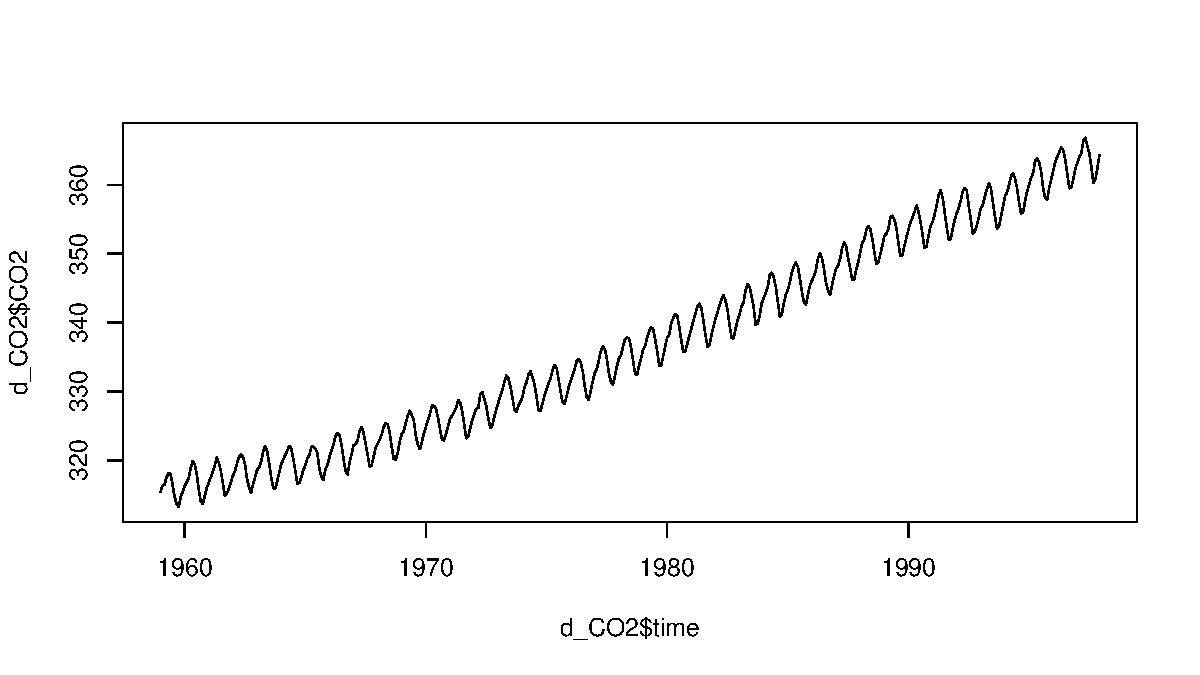
\includegraphics[width=576px]{bookdown-demo_files/figure-latex/unnamed-chunk-56-1}

\begin{center}\rule{0.5\linewidth}{0.5pt}\end{center}

\hypertarget{ux4feeux6539ux989cux8272ux8bbeux7f6e}{%
\subsection{修改颜色设置}\label{ux4feeux6539ux989cux8272ux8bbeux7f6e}}

\begin{Shaded}
\begin{Highlighting}[]
\FunctionTok{plot}\NormalTok{(}\AttributeTok{x =}\NormalTok{ d\_CO2}\SpecialCharTok{$}\NormalTok{time, }\AttributeTok{y =}\NormalTok{ d\_CO2}\SpecialCharTok{$}\NormalTok{CO2, }\AttributeTok{type =} \StringTok{"l"}\NormalTok{, }\AttributeTok{col =} \StringTok{"red"}\NormalTok{)}
\end{Highlighting}
\end{Shaded}

.pull-right{[}

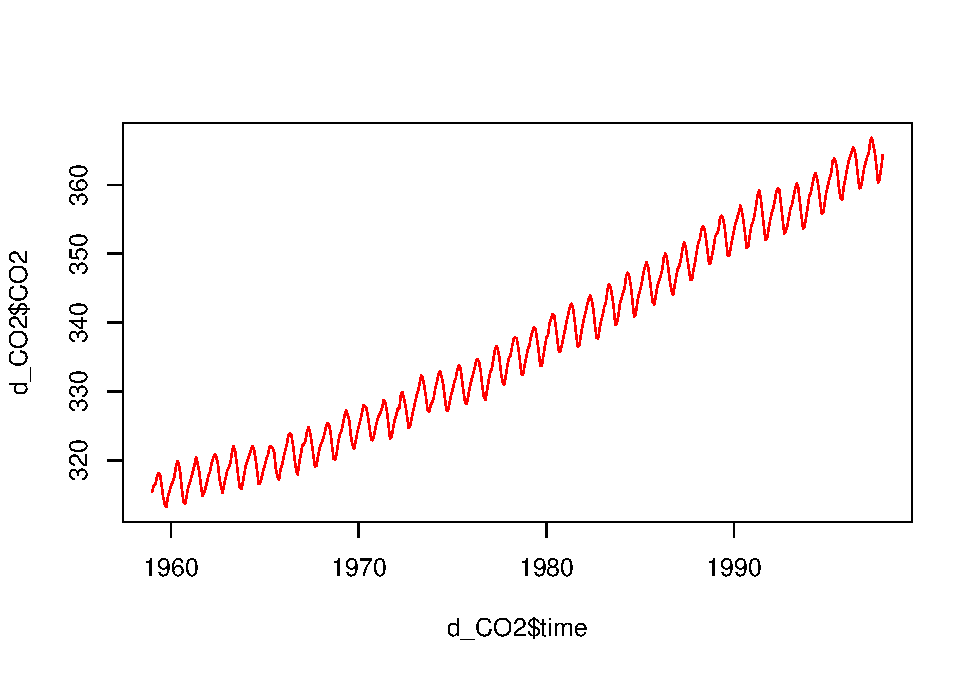
\includegraphics[width=576px]{bookdown-demo_files/figure-latex/unnamed-chunk-57-1}

\hypertarget{ux4feeux6539ux5750ux6807ux8f74ux540dux79f0}{%
\subsection{修改坐标轴名称}\label{ux4feeux6539ux5750ux6807ux8f74ux540dux79f0}}

\begin{Shaded}
\begin{Highlighting}[]
\FunctionTok{plot}\NormalTok{(}\AttributeTok{x =}\NormalTok{ d\_CO2}\SpecialCharTok{$}\NormalTok{time, }\AttributeTok{y =}\NormalTok{ d\_CO2}\SpecialCharTok{$}\NormalTok{CO2, }\AttributeTok{type =} \StringTok{"l"}\NormalTok{, }\AttributeTok{col =} \StringTok{"red"}\NormalTok{, }\AttributeTok{xlab =} \StringTok{"Year"}\NormalTok{, }\AttributeTok{ylab =} \FunctionTok{expression}\NormalTok{(pCO[}\DecValTok{2}\NormalTok{]}\SpecialCharTok{\textasciitilde{}}\StringTok{"(ppm)"}\NormalTok{))}
\end{Highlighting}
\end{Shaded}

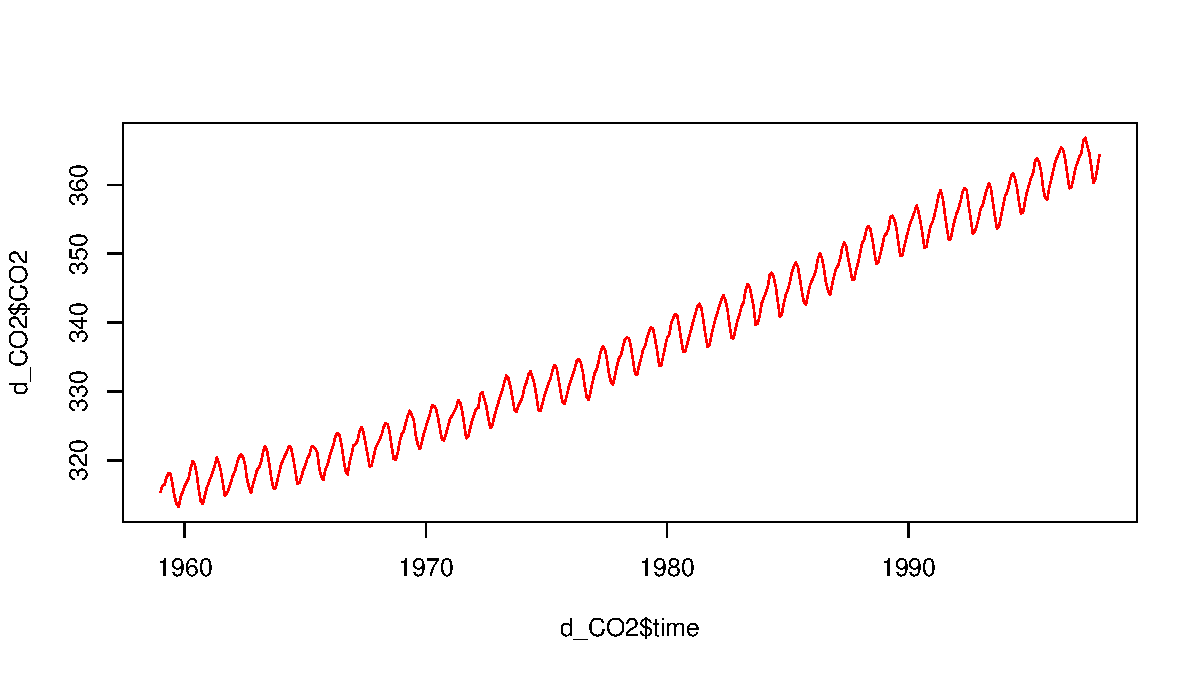
\includegraphics[width=576px]{bookdown-demo_files/figure-latex/unnamed-chunk-58-1}

\hypertarget{ggplotux4f5cux56fe}{%
\section{\texorpdfstring{\texttt{ggplot}作图}{ggplot作图}}\label{ggplotux4f5cux56fe}}

先对\texttt{ggplot}绘图有个简单印象,下次课我们深入学习。

\begin{Shaded}
\begin{Highlighting}[]
\FunctionTok{library}\NormalTok{(ggplot2) }\CommentTok{\#ggplot绘图}
\FunctionTok{ggplot}\NormalTok{(d\_CO2, }\FunctionTok{aes}\NormalTok{(time, CO2))}\SpecialCharTok{+}
  \FunctionTok{theme\_bw}\NormalTok{()}\SpecialCharTok{+}
  \FunctionTok{geom\_line}\NormalTok{(}\AttributeTok{color =} \StringTok{"red2"}\NormalTok{)}\SpecialCharTok{+}
  \FunctionTok{labs}\NormalTok{(}\AttributeTok{x =} \StringTok{"Year"}\NormalTok{,}
       \AttributeTok{y =} \SpecialCharTok{\textasciitilde{}}\NormalTok{pCO[}\DecValTok{2}\NormalTok{]}\SpecialCharTok{\textasciitilde{}}\NormalTok{(ppm))}
\end{Highlighting}
\end{Shaded}

\begin{verbatim}
## Don't know how to automatically pick scale for object of type ts. Defaulting to continuous.
## Don't know how to automatically pick scale for object of type ts. Defaulting to continuous.
\end{verbatim}

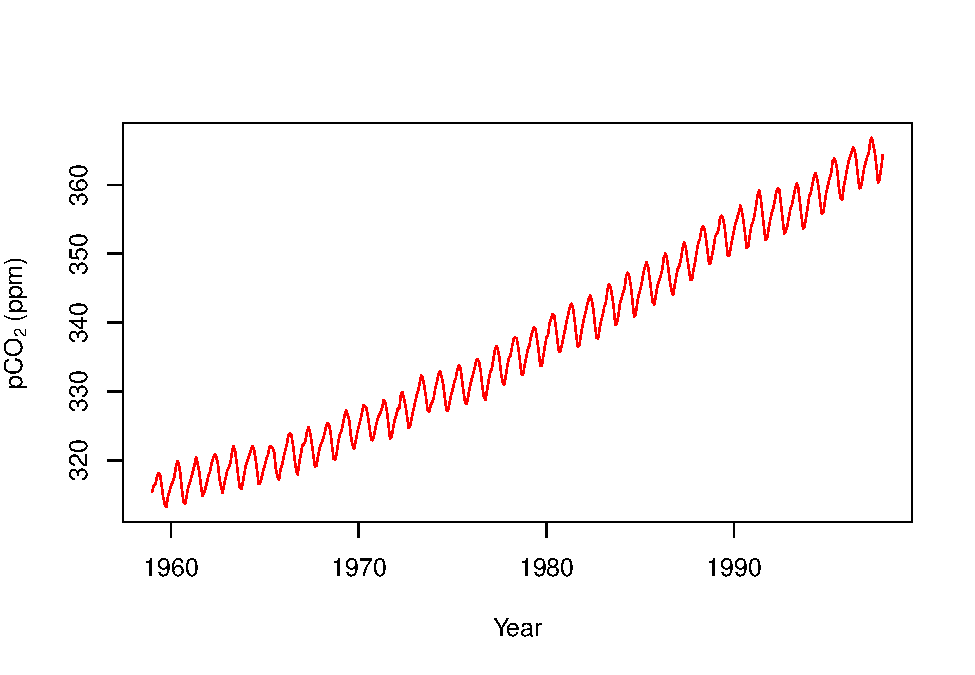
\includegraphics{bookdown-demo_files/figure-latex/unnamed-chunk-59-1.pdf}

\begin{Shaded}
\begin{Highlighting}[]
\CommentTok{\#ggsave("pCO2.png", width=342/90, height=243/90, dpi=600)}
\end{Highlighting}
\end{Shaded}

\hypertarget{ux4fddux5b58ux56feux7247}{%
\section{保存图片}\label{ux4fddux5b58ux56feux7247}}

\hypertarget{ux7b2cux4e00ux79cdux65b9ux6cd5}{%
\subsection{第一种方法}\label{ux7b2cux4e00ux79cdux65b9ux6cd5}}

首先将图片赋值给变量\textbf{\texttt{p1}}。

\begin{Shaded}
\begin{Highlighting}[]
\FunctionTok{library}\NormalTok{(ggplot2)}

\NormalTok{p1 }\OtherTok{\textless{}{-}} \FunctionTok{ggplot}\NormalTok{(mpg, }\FunctionTok{aes}\NormalTok{(displ, hwy))}\SpecialCharTok{+}
  \FunctionTok{geom\_point}\NormalTok{()}


\NormalTok{然后调用}\SpecialCharTok{**}\StringTok{\textasciigrave{}}\AttributeTok{png()}\StringTok{\textasciigrave{}}\SpecialCharTok{**}\NormalTok{作图设备作图,并记得随手用}\SpecialCharTok{**}\StringTok{\textasciigrave{}}\AttributeTok{dev.off()}\StringTok{\textasciigrave{}}\SpecialCharTok{**}\NormalTok{关闭作图设备(否则不出图)。变量}\SpecialCharTok{**}\StringTok{\textasciigrave{}}\AttributeTok{p1}\StringTok{\textasciigrave{}}\SpecialCharTok{**}\NormalTok{夹在以上两行代码之间。完成操作后,你就能在工作文件夹里找到名称为“myplot\_1.png”的图了。}

\StringTok{\textasciigrave{}\textasciigrave{}\textasciigrave{}}\AttributeTok{r }
\AttributeTok{png("myplot\_1.png", width=359/90*600, height=239/90*600, res=600)}
\AttributeTok{p1}
\AttributeTok{dev.off()}
\end{Highlighting}
\end{Shaded}

\hypertarget{ux4fddux5b58ux56feux7247-1}{%
\section{保存图片}\label{ux4fddux5b58ux56feux7247-1}}

\hypertarget{ux7b2cux4e8cux79cdux65b9ux6cd5}{%
\subsection{第二种方法}\label{ux7b2cux4e8cux79cdux65b9ux6cd5}}

由于我们以后大多使用\textbf{\texttt{ggplot()}}作图,因此可以用\textbf{\texttt{ggplot2}}程序包中的\textbf{\texttt{ggsave()}}函数保存当前显示的图片(在RStudio右下面板中)。

\begin{Shaded}
\begin{Highlighting}[]
\FunctionTok{library}\NormalTok{(ggplot2)}
\FunctionTok{ggplot}\NormalTok{(mpg, }\FunctionTok{aes}\NormalTok{(displ, hwy))}\SpecialCharTok{+}
  \FunctionTok{geom\_point}\NormalTok{()}

\FunctionTok{ggsave}\NormalTok{(}\StringTok{"myplot\_2.png"}\NormalTok{, }\AttributeTok{width=}\DecValTok{359}\SpecialCharTok{/}\DecValTok{90}\NormalTok{, }\AttributeTok{height=}\DecValTok{239}\SpecialCharTok{/}\DecValTok{90}\NormalTok{, }\AttributeTok{dpi=}\DecValTok{600}\NormalTok{) }\CommentTok{\#png格式,位图}
\FunctionTok{ggsave}\NormalTok{(}\StringTok{"myplot\_2.pdf"}\NormalTok{, }\AttributeTok{width=}\DecValTok{359}\SpecialCharTok{/}\DecValTok{90}\NormalTok{, }\AttributeTok{height=}\DecValTok{239}\SpecialCharTok{/}\DecValTok{90}\NormalTok{) }\CommentTok{\#pdf格式,矢量图}
\end{Highlighting}
\end{Shaded}

完成以上操作,你就能在工作文件夹里找到名称为``myplot\_2.png''``myplot\_2.pdf''的图了。

\begin{quote}
如何设置合适的\textbf{\texttt{width}}和\textbf{\texttt{height}}?\\
需要一些技巧(我会操作演示)和审美能力。
\end{quote}

\begin{center}\rule{0.5\linewidth}{0.5pt}\end{center}

\hypertarget{ux63a8ux8350ux9605ux8bfb}{%
\section{推荐阅读}\label{ux63a8ux8350ux9605ux8bfb}}

Crawley MJ. The R Book. 2nd ed.~Chapter 2. Essentials of the R Language.pp 12-136.
(有点枯燥,至少读1/3,读不完的之后的学习过程中还可以再回过头读。)

\hypertarget{ggplot2ux4f5cux56feux5165ux95e8}{%
\chapter{\texorpdfstring{\texttt{ggplot2}作图入门}{ggplot2作图入门}}\label{ggplot2ux4f5cux56feux5165ux95e8}}

Here is a review of existing methods.

\hypertarget{ux6570ux636eux6574ux7406}{%
\chapter{数据整理}\label{ux6570ux636eux6574ux7406}}

We describe our methods in this chapter.

Math can be added in body using usual syntax like this

\hypertarget{math-example}{%
\section{math example}\label{math-example}}

\(p\) is unknown but expected to be around 1/3. Standard error will be approximated

\[
SE = \sqrt(\frac{p(1-p)}{n}) \approx \sqrt{\frac{1/3 (1 - 1/3)} {300}} = 0.027
\]

You can also use math in footnotes like this\footnote{where we mention \(p = \frac{a}{b}\)}.

We will approximate standard error to 0.027\footnote{\(p\) is unknown but expected to be around 1/3. Standard error will be approximated

  \[
  SE = \sqrt(\frac{p(1-p)}{n}) \approx \sqrt{\frac{1/3 (1 - 1/3)} {300}} = 0.027
  \]}

\hypertarget{lubridateux5904ux7406ux65f6ux95f4ux6570ux636e}{%
\chapter{\texorpdfstring{\texttt{lubridate}处理时间数据}{lubridate处理时间数据}}\label{lubridateux5904ux7406ux65f6ux95f4ux6570ux636e}}

Some \emph{significant} applications are demonstrated in this chapter.

\hypertarget{example-one}{%
\section{Example one}\label{example-one}}

\hypertarget{example-two}{%
\section{Example two}\label{example-two}}

\hypertarget{ux7ed8ux5236ux5730ux56fe}{%
\chapter{绘制地图}\label{ux7ed8ux5236ux5730ux56fe}}

We have finished a nice book.

\hypertarget{ux76f8ux5173ux6027ux5206ux6790}{%
\chapter{相关性分析}\label{ux76f8ux5173ux6027ux5206ux6790}}

Here is a review of existing methods.

\hypertarget{ux7ebfux6027ux56deux5f52}{%
\chapter{线性回归}\label{ux7ebfux6027ux56deux5f52}}

Here is a review of existing methods.

\hypertarget{logisticux56deux5f52}{%
\chapter{Logistic回归}\label{logisticux56deux5f52}}

Here is a review of existing methods.

\hypertarget{tux68c0ux9a8c}{%
\chapter{\texorpdfstring{\emph{t}检验}{t检验}}\label{tux68c0ux9a8c}}

Here is a review of existing methods.

\hypertarget{ux5355ux56e0ux7d20ux65b9ux5deeux5206ux6790}{%
\chapter{单因素方差分析}\label{ux5355ux56e0ux7d20ux65b9ux5deeux5206ux6790}}

Here is a review of existing methods.

\hypertarget{ux591aux56e0ux7d20ux65b9ux5deeux5206ux6790}{%
\chapter{多因素方差分析}\label{ux591aux56e0ux7d20ux65b9ux5deeux5206ux6790}}

Here is a review of existing methods.

\hypertarget{ux534fux65b9ux5deeux5206ux6790}{%
\chapter{协方差分析}\label{ux534fux65b9ux5deeux5206ux6790}}

Here is a review of existing methods.

\hypertarget{ux4e3bux6210ux5206ux5206ux6790}{%
\chapter{主成分分析}\label{ux4e3bux6210ux5206ux5206ux6790}}

Here is a review of existing methods.

  \bibliography{book.bib,packages.bib}

\end{document}
